\section{System Architecture}
\label{sec:architecture}
\label{sec:framework}
\label{sec:methodology}

In this section we present a high-level overview of the proposed system and detail its components and algorithms. The architecture composes the four primitives of Section~\ref{sec:preliminaries} into one end-to-end pipeline. Fig.~\ref{fig:architecture} shows the two phases and the JSON artifact that connects them.

\begin{figure*}[t]
  \centering
  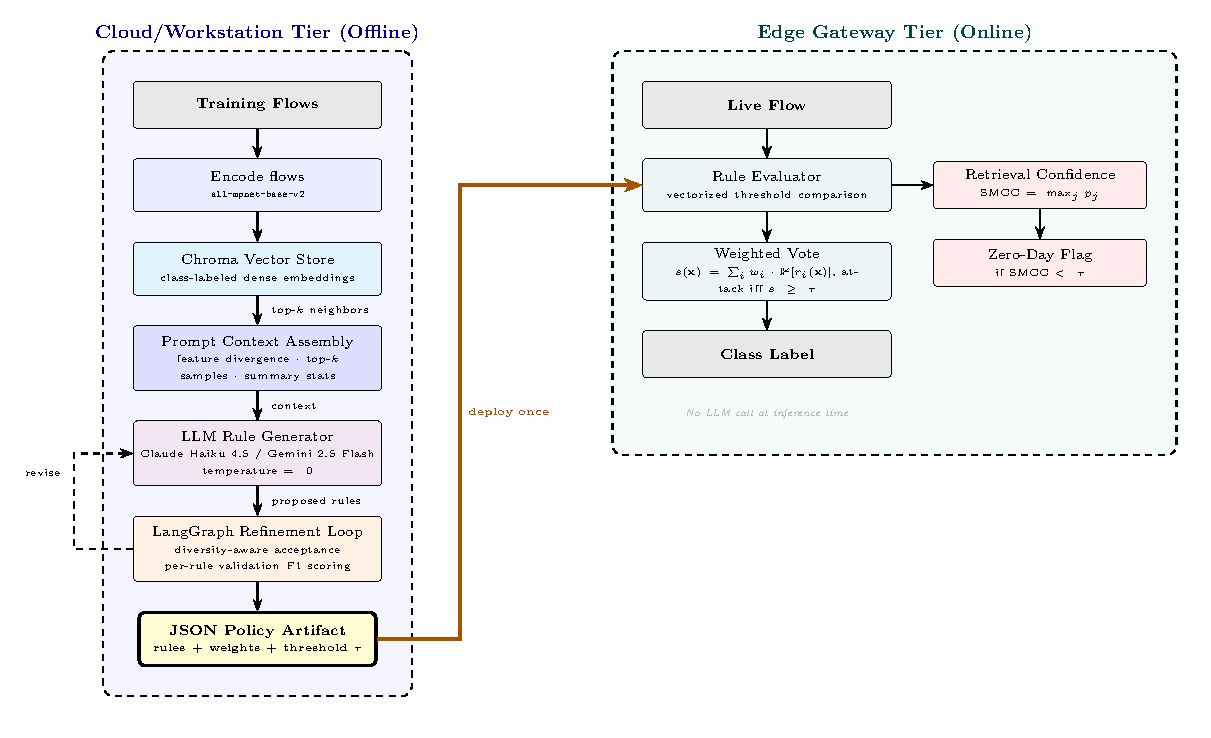
\includegraphics[width=\linewidth]{figures/fig_architecture.pdf}
  \caption{End-to-end architecture. Offline (left) the system embeds training flows into a Chroma vector store, retrieves class-representative neighbors by mean-embedding cosine similarity, and prompts Claude Haiku 4.5 to emit JSON threshold rules. A LangGraph refinement loop iterates on per-rule validation F1. Online (right) the deployed rule evaluator scores each flow with a vectorized threshold comparison and a weighted vote. No language-model call is required at inference time.}
  \label{fig:architecture}
\end{figure*}

The architecture follows a two-tier split mirroring the end-edge-cloud
structure of AIoT systems. The cloud or workstation tier carries the heavy
reasoning: it embeds traffic, retrieves evidence, and drives an agentic
refinement loop that synthesizes the policy. The edge tier carries the
detection, applying a stateless evaluator to live flows at line rate. The split
pays the expensive computation once while keeping the gateway runtime within an
embedded budget. The remainder of this section describes each tier, the
policy-generation protocol, and the four evaluation protocols that exercise the
architecture.

\subsection{Cloud and Workstation Tier}
\label{subsec:offline}

The cloud tier performs offline policy synthesis once per dataset and never
touches the gateway at inference time, hosting every cost a constrained device
cannot afford---the embedding model, vector store, language model, and
refinement loop---across five stages.

\begin{enumerate}
  \item \textit{Featurization and embedding.} Each flow is encoded into the dataset's numeric schema, embedded with sentence-transformers/all-mpnet-base-v2, and persisted in a Chroma vector store under its class label.
  \item \textit{Evidence retrieval.} A mean embedding is computed per class and the top-$k$ nearest neighbors are retrieved by cosine similarity (Eq.~\ref{eq:cosine}), forming a class-representative sample within the language-model context window.
  \item \textit{Feature divergence ranking.} Permutation importance (Eq.~\ref{eq:permimp}) and the standardized mean difference (Eq.~\ref{eq:cohend}) rank the input features; the top-ranked names and summary statistics form the prompt context.
  \item \textit{Rule synthesis.} The language model is queried at temperature zero and emits threshold rules as JSON tuples (feature\_name, op, value, target\_class) deployable as ACL-style firewall entries.
  \item \textit{Agentic refinement.} A LangGraph state machine scores each proposed rule on the validation slice, returns per-rule F1 as tool output, steers the model toward uncovered detection phenomena, and retains the best-scoring policy across rounds.
\end{enumerate}
All five stages run offline; no model weights or embeddings are shipped to the
edge.

\subsection{Edge Gateway Tier}
\label{subsec:online}

The deployed component is a stateless rule evaluator. It scores each encoded
flow by evaluating every threshold rule as a vectorized comparison and
combining the fired rules through a weighted vote. No model weights, embeddings,
or language-model calls run at inference time; the policy is a small JSON file
mapping directly onto ACL-style firewall entries, which keeps the evaluator
portable across IoT gateway hardware. The same evaluator also exposes the
retrieved-neighbor confidence as an out-of-distribution signal.

\subsection{System Overview}
\label{subsec:overview}

As shown in Fig.~\ref{fig:architecture}, the workflow chains the two tiers. The
cloud tier featurizes and embeds the training split, ranks features by
normal-versus-attack divergence to build the prompt context, and runs the
refinement loop---proposing phenomenon-tagged rules, accepting a diverse
subset, and calibrating per-rule weights and the vote threshold---before
serializing one JSON policy artifact. The gateway then loads that artifact and
scores each live flow with a vectorized threshold comparison and weighted vote,
reporting the retrieval-confidence score as a zero-day flag. The cloud stages
run once and the gateway stages run continuously, so the language-model cost is
paid a single time and the gateway carries no learned parameters.


\subsection{Policy Generation Protocol}
\label{subsec:policy_generation}

The policy-generation loop is the core of the architecture and is common to
every downstream evaluation. It runs entirely client-side at the cloud tier
and emits a single policy JSON artifact per run, which is the only object
shipped to the gateway. The language-model generator is a swappable component:
any vendor's model can drive the loop without changing the surrounding
retrieval, acceptance, and voting stages. Global hyperparameters are fixed at
$k_{\text{rules}}=5$, $n_{\text{top}}=5$, and $n_{\text{rounds}}=8$.

\paragraph{Class-balanced corpora.}
For each dataset we sample at most $C = \min(N_{\text{normal}},
N_{\text{attack}}, C_{\max})$ flows per class, where $C_{\max}$ is a
per-dataset cap that bounds the language-model context size. Each corpus is
divided by a stratified 80/20 train/test split, with a 20\% validation slice
carved off the training set; the held-out test set is observed only once, at
the end of the loop.

\paragraph{Stats package and prompt context.}
Per-feature normal-versus-attack divergence is ranked by the standardized mean
difference of Eq.~\ref{eq:cohend}, and the top $n_{\text{top}}$ features form
the context the language model consumes. The human prompt presents three
elements: the global attack-versus-normal mean, std, p10, median, and p90 for
each top feature; the per-attack-class means for the same features when class
labels are available, which supplies the cross-class generalization signal;
and value-count overviews for low-cardinality categorical columns.

\paragraph{Phenomenon-tagged rule proposals.}
Each round the language model emits exactly $k_{\text{rules}}=5$ rules through
a structured propose-rule tool. Every proposal carries five fields: a feature;
an operator from $\{<, \leq, >, \geq, ==, \neq\}$, with equality on continuous
floats explicitly prohibited; a numeric or categorical value; a
controlled-vocabulary phenomenon tag from
$\{$Handshake, Asymmetry, Timing, Header, Service, State, Volume, Entropy$\}$;
and a one-sentence rationale. The phenomenon vocabulary tells the next round
which protocol-level concepts the current policy already covers, steering the
model toward uncovered phenomena and away from per-feature clones.

\paragraph{Diversity-aware acceptance.}
After scoring every candidate rule's per-rule F1 on the validation slice, the
$k$ accepted rules are filled greedily by a composite score
\[
  S(r \mid A) = \alpha \cdot \mathrm{F1}_{\text{val}}(r)
  + (1 - \alpha) \cdot D(r \mid A),
\]
where $A$ is the already-accepted set and the diversity term decomposes as
\[
\begin{aligned}
D(r \mid A) &= w_t \cdot \mathrm{tag}(r,A)
  + w_d \cdot \mathrm{dis}(r,A) \\
&\quad + w_f \cdot \mathrm{feat}(r,A)
  + w_\theta \cdot \mathrm{thr}(r,A).
\end{aligned}
\]
\textit{tag} is one minus the fraction of $A$ already carrying $r$'s
phenomenon tag. \textit{feat} indicates feature novelty. \textit{thr}
measures threshold separation when the feature is re-used. \textit{dis} is an
imbalance-aware decision disagreement,
$1 - (J_{\text{normal}} + J_{\text{attack}})/2$, with $J_{\text{class}}$ the
Jaccard similarity of fire-sets computed \emph{within} each class. The
per-class decomposition prevents the metric from collapsing to triviality on
severely imbalanced datasets where any two attack-predicting rules agree on
nearly all rows. Default weights are $\alpha = 0.6$ and
$(w_t, w_d, w_f, w_\theta) = (0.35, 0.30, 0.20, 0.15)$.

\paragraph{Weighted voting with calibrated threshold.}
At inference time the policy applies each rule independently to a flow and
combines the binary outputs through a weighted vote
$s(\mathbf{x}) = \sum_i w_i \cdot \mathbb{1}[r_i(\mathbf{x})]$. It classifies
$\mathbf{x}$ as attack iff $s(\mathbf{x}) \geq \tau$. Per-rule weights are the
per-rule attack-class precision on the validation slice. The threshold $\tau$
is auto-calibrated on the same slice to maximize the selected metric. The
default metric is macro-averaged F1, and alternatives include attack-class F1
and attack precision at recall $\geq 0.9$. Both $\{w_i\}$ and $\tau$ are
serialized inside the policy JSON, so the canonical evaluator reproduces any
metric exactly without re-running the language model.

\paragraph{Round selection and early stopping.}
The loop runs for up to $n_{\text{rounds}} = 8$ rounds. It early-stops when the
validation selected-metric does not improve for two consecutive rounds. The
round selected for reporting is the one with the highest validation-slice
score. The test split is never observed during selection. Algorithm~\ref{alg:synthesis}
states the full loop.

\begin{algorithm}[t]
\caption{Offline Policy Synthesis}
\label{alg:synthesis}
\begin{algorithmic}[1]
\Require Balanced corpus $\mathcal{D}$, feature statistics, $n_{\text{rounds}}$, $k_{\text{rules}}$
\Ensure Policy $\pi$ with weights $\{w_i\}$ and threshold $\tau$
\State Build prompt context from the top $n_{\text{top}}$ divergence-ranked features
\State $\pi_{\text{best}} \gets \varnothing$,\ \ $s_{\text{best}} \gets 0$,\ \ $\text{cov} \gets \varnothing$
\For{$\text{round} = 1$ to $n_{\text{rounds}}$}
  \State $\mathcal{C} \gets \textsc{Propose}(k_{\text{rules}}\ \text{rules} \mid \text{context}, \text{cov})$
  \For{each candidate $r \in \mathcal{C}$}
    \State compute $\mathrm{F1}_{\text{val}}(r)$ on the validation slice
  \EndFor
  \State $A \gets$ greedy selection of $k$ rules maximizing $S(r \mid A)$
  \State calibrate $\{w_i\}$ and $\tau$ on the validation slice
  \State $s \gets$ selected-metric of $A$ on the validation slice
  \If{$s > s_{\text{best}}$}
    \State $\pi_{\text{best}} \gets A$,\ \ $s_{\text{best}} \gets s$
  \EndIf
  \State $\text{cov} \gets$ phenomenon tags covered by $A$
  \If{no improvement for two consecutive rounds}
    \State \textbf{break}
  \EndIf
\EndFor
\State serialize $\pi_{\text{best}}$ with $\{w_i\}$ and $\tau$ to JSON
\State \Return $\pi_{\text{best}}$
\end{algorithmic}
\end{algorithm}

\subsection{Multi-Class Classification Protocol}
\label{subsec:multiclass}

Multi-class classification reuses the policy loop with three changes. Labels
are stored alongside feature vectors in the Chroma store so that retrieved
neighbors carry class provenance. The prompt lists the complete set of $K$
known attack classes, and majority voting over the top-$k$ retrieved neighbors
supplies a soft class prior as in-context evidence. The generator then
synthesizes one decision-rule vector per class, each with $k_{\text{rules}}=5$
threshold conditions over the top-$n_{\text{top}}$ permutation-importance
features, emitted as the same JSON tuples deployable as ACL-style firewall
entries.

\subsection{Zero-Day Detection Protocol}
\label{subsec:zeroday}

Rule-based detectors are closed-set by construction and cannot name a truly
novel attack class. This protocol tests whether retrieval confidence degrades
gracefully on out-of-distribution traffic, enabling an anomaly flag without a
matching rule. For each dataset a designated withheld class $c^{*}$ is removed
from the training split and the Chroma store, leaving the remaining $K-1$
classes as the closed-set regime; the $c^{*}$ flows are reintroduced at
inference time alongside balanced known-class samples. Rather than labeling
unseen traffic, we monitor the retrieved-neighbor distribution: with $p_j$ the
proportion of retrieved neighbors of class $j$, the soft-max class-confidence
(SMCC) score is
\[
  \mathrm{SMCC}(\mathbf{x}) = \max_{j \in \mathcal{K}} p_j
\]
over the known classes $\mathcal{K}$. A query with
$\mathrm{SMCC}(\mathbf{x}) < \tau$ is flagged as a candidate zero-day event.
Sweeping $\tau$ from $0$ to $1$ traces the Zero-Day Detection Rate (ZDR) and
False Positive Rate reported in \S\ref{subsec:threshold}, where
$\mathrm{ZDR} = \mathrm{TP}_{c^{*}} / |\mathcal{D}_{c^{*}}|$ is the fraction of
withheld-class flows correctly flagged.

\subsection{Anonymization Ablation}
\label{subsec:anon}

The prompt necessarily exposes raw feature names (e.g., Header\_Length,
SrcAddr), which can leak deployment topology or vendor information. This
ablation tests whether replacing semantic names with opaque identifiers
degrades detection. For each dataset a fixed bijective map
$\sigma: \text{feature\_name} \to f_i$ relabels every feature, so the model
sees only opaque identifiers and numeric values. We compare an \emph{Original}
condition (semantic names) against an \emph{Anonymized} condition (opaque
identifiers), reporting the utility cost
$\Delta F1 = \overline{F1}_{\text{anon}} - \overline{F1}_{\text{orig}}$ on a
held-out test set and the Jaccard overlap of the selected feature sets,
\[
  J = \frac{\left| \mathcal{F}_{\text{orig}} \cap \mathcal{F}_{\text{anon}} \right|}
           {\left| \mathcal{F}_{\text{orig}} \cup \mathcal{F}_{\text{anon}} \right|} .
\]

\subsection{Adversarial Robustness Protocol}
\label{subsec:kerckhoffs}

The robustness protocol adopts the Kerckhoffs principle: the attacker has full
knowledge of the rule set and applies the minimum feature perturbation needed
to evade detection. The budget $\varepsilon$ is expressed as a fraction of each
feature's interquartile range, and the adversary perturbs withheld-class flows
toward the nearest known-class centroid. The Exploitability Sweep Rate is the
fraction of originally-flagged flows that evade at budget $\varepsilon$,
\[
  \mathrm{ESR}(\varepsilon) = \frac{\text{flows that evade at budget } \varepsilon}
                                   {\text{flows flagged at } \varepsilon = 0} ,
\]
and the summary metric is the critical budget $\varepsilon_{0.5}$ at which
$\mathrm{ESR}=0.5$, quantifying each detector's adversarial hardness. The LLM
policy is compared against Decision Tree and Random Forest baselines under this
sweep (Table~\ref{tab:kerckhoffs}).

Together these protocols define the operating envelope of the architecture.
Section~\ref{sec:resultsAndDisc} applies them across the five IoT benchmarks
and reports closed-set accuracy, cross-vendor agreement, synthesis cost, the
zero-day extension, adversarial hardness, and edge latency on Raspberry Pi
hardware.
